\documentclass[natbib]{svjour3}

% UTF8 support
\usepackage[utf8x]{inputenc}

\usepackage[english]{babel}


\usepackage{graphicx}
\graphicspath{{figs/}}

\usepackage{amsmath}

\usepackage{tikz}
\usetikzlibrary{shapes}

\usepackage{hyperref}
\usepackage{subcaption}

\usepackage[draft, footnote, margin=false]{fixme}

\newcommand{\ie}{{\textit{i.e.\ }}}
\newcommand{\cf}{{\textit{cf\ }}}
\newcommand{\eg}{{\textit{e.g.\ }}}
\newcommand{\al}{{\textit{et al.\ }}}

\newcommand{\M}[3]{{\mathcal{M}(#1, #2, #3)}}
\newcommand{\model}[3]{{$\mathcal{M}(#1, #2, #3)$}}
% generic mutual model (gmodel) 
\newcommand{\gmodel}[2]{{$\mathcal{M}(#1, #2)$}}
\newcommand{\Gmodel}[2]{{\mathcal{M}(#1, #2)}}
\newcommand{\refmodel}[2]{{$\mathcal{M}(#1, #2)$}}
\newcommand{\Model}[3]{{$\mathcal{M}^{\circ}(#1, #2, #3)$}}
\newcommand{\gModel}[2]{{$\mathcal{M}^{\circ}(#1, #2)$}}
\newcommand{\Mdeg}[3]{{\mathcal{M}^{\circ}(#1, #2, #3)}}
\newcommand{\gMdeg}[2]{{\mathcal{M}^{\circ}(#1, #2)}}

\newcommand{\groundingcriterion}{{$\mathcal{M}^{\circ}_{min}$}}
\newcommand{\inigrounding}{{$\mathcal{M}^{\circ}_{t_0}$}}

\newcommand{\concept}[1]{{\small \texttt{#1}}}
\newcommand{\stmt}[1]{{\footnotesize \tt $\langle$ #1\relax$\rangle$}}

\usepackage{mathtools}
\DeclarePairedDelimiter\abs{\lvert}{\rvert}%
\newcommand*\mean[1]{\overline{#1}}

\title{Mutual Modelling}

\author{
    Pierre Dillenbourg
    \and
    Séverin Lemaignan
    \and
    Nicolas Nova
    \and
    Gaëlle Molinari
}
\institute{
    Pierre Dillenbourg, Séverin Lemaignan \at Computer-Human Interaction in Learning and Instruction \\
    École Polytechnique Fédérale de Lausanne (EPFL) \\ CH-1015 Lausanne, Switzerland \\
    \email{firstname.lastname@epfl.ch}
    \and
    Nicolas Nova \at Haute École Arts \& Design de Genève \\ CH-1201 Genève, Switzerland\\\email{nicolas.nova@hesge.ch}
    \and
    Gaëlle Molinari \at Distance Learning University Switzerland (Unidistance),
    CH-3960 Sierre, Switzerland\\\email{gaelle.molinari@unidistance.ch}
}
\begin{document}
\maketitle

\begin{abstract}
    Collaborative learning has something to do with building a shared
    understanding of the situation at hand. Yet, the psycholinguistics mechanisms
    at work while establishing common grounds are complex and certainly involve
    modelling what the partner knows/wants/intends at a given time.

    Building on a set of five independent studies that where conducted over
    several years, we propose in this article a simple model of the mechanisms
    of mutual modelling. It integrates several concepts related to the classical
    idea of grounding, and we apply it as an operational tool to
    analyse the interplay of learning and mutual modelling in the five studies.

    We come up with mixed experimental results that evidence the dual nature of
    mutual modelling: a individual meta-cognitive aptitude that co-exists with
    modelling elicited and fostered by social interactions.

\end{abstract}

\section{Introduction}


From its very beginning, CSCL research has been following
\citet{roschelle1995construction} suggestion that collaborative learning has
something to do with the process of constructing and maintaining a \emph{shared
understanding} of the task at hand. Building a shared/mutual understanding
refers to the upper class of collaborative learning situations, those in which
students should build upon each other's understanding to refine their own
understanding: what is expected to produce learning is not the mere fact that
two students build the same understanding but the cognitive effort they have to
engage to build this shared understanding~\citep{schwartz1995emergence}. This
effort can be observed by the frequency of rich interactions, \ie interactions
whose occurrence has been related to learning: (self-) explanations in cognitive
science~\citep{chi1989self, webb1991task}, conflict resolution in
socio-cognitive theories~\citep{doise1975social},
mutual regulation~\citep{blaye1995collaborative} in a Vygostkian perspective, etc. The
construction of a shared understanding has been investigated for several years
in psycholinguistics, under the  notion of
\emph{grounding}~\citep{clark1986referring}. However, the relevance of grounding
mechanisms for explaining learning outcomes has been questioned in learning
sciences. The monitoring and repair of misunderstanding explains for instance
referential failures in short dialogue episodes but does hardly predict
\emph{conceptual change} (\ie the acquisition, acceptation and integration of a
new belief into one's mental model) over longer
sessions~\citep{dillenbourg2006sharing}. The cumulative effect of grounding
episodes can probably be better understood from a socio-cultural perspective:

\begin{quote}
Collaborative learning is associated with the increased
cognitive-interactional effort involved in the transition from \emph{learning to
understand each other} to \emph{learning to understand the meanings of the semiotic
tools that constitute the mediators of interpersonal
interaction}~\citep{baker1999role}
\end{quote}

Along this line, several scholars suggest that CSCL research should go deeper in
the understanding of how partners engage into shared meaning
making~\citep{stahl2007meaning} or \emph{intersubjective} meaning
making~\citep{suthers2006technology}.

Paradoxically, while Clark's theory is somewhat too linguistic from a conceptual
change viewpoint, it is criticized at the same time as being too cognitivist by
some psycholinguists, \ie as overestimating the amount of shared knowledge and
mutual representations actually necessary to conduct a dialogue. The fundamental
issue, as old as philosophy, is the degree of coupling between the different
levels of dialogue, mostly between the lexical/syntactical level and the deeper
semantic levels. \citet{pickering2006alignment} argue that the mutual
understanding starts mostly with a \emph{superficial alignment} at the level of
the linguistic representations, due to priming mechanisms, and that this local
alignment may -- in some cases -- lead to a \emph{global alignment} of the
semantic level (\emph{deep grounding}).  For these authors, the convergence in
dialogue, and even the repair of some misunderstandings, is explained by this
mimetic behavior more than by a monitoring of each other's knowledge:
\emph{``...interlocutors do not need to monitor and develop full common ground
as a regular, constant part of routine conversation, as it would be
unnecessary and far too costly. Establishment of full common ground is, we
argue, a specialized and non-automatic process that is used primarily in
times of difficulty (when radical misalignment becomes apparent).''} (p. 179).
This view is actually not incompatible with Clark's \emph{grounding
criterion}~\citep{clark1989contributing}: the degree of shared understanding that
peers need to reach depends upon the task they perform. For instance, a dialogue
between two surgeons might rely on superficial alignment if they talk about
their friends but has to guarantee accurate common grounds when talking about
which intervention will be conducted in which way on which patient. 
%Some CSCL
%scholars stressed the ``illusion of shared understanding'' \fixme{REF: Jacco?},
%\ie the potential decoupling between linguistic alignment and actual shared
%meanings.

This interesting cognitive science debate occurred mostly outside the field of
learning. In education, the question is to relate these mechanisms to learning
outcomes: \textbf{Is linguistic alignment sufficient to trigger conceptual
change?} \textbf{Does negotiation of meaning only occurs when partners monitor
and diagnose each other's knowledge?} If the ratio between shallow alignment and
deep grounding depends upon the task, and if deep grounding is a condition for
learning, then the pedagogical challenge is indeed to design tasks that require
deep grounding. Most empirical studies on grounding and alignment are conducted
with tasks, which despite being qualified as ``ecologically valid'' by their
authors, are mere referencing tasks such as asking the way to the train station
or helping the peer to choose a picture among many. In this contribution, we
explore several richer tasks such as arguing on a sensitive issue or building a
concept map.  

Deep grounding or shared meaning making requires some cognitive load. For
\citet{clark1986referring}, what is important is not the individual effort made
by the receiver of a communicative act, but the overall \emph{least collaborative
effort}.  The cost of producing a perfect utterance may be higher than the cost
of repairing the problems that may arise through misunderstandings, and in fact,
subjects tend to make less efforts adapting their utterances to a specific
partner when they know that they can later provide feedback on his/her
understanding~\citep{schober1993spatial}. We introduced the notion of
\emph{optimal collaborative effort}~\citep{dillenbourg1995evolution} to stress
that misunderstanding should not be viewed as something to be avoided (if this
was possible), but as an opportunity to engage into verbalization, explanation,
negotiation, and so forth. This issue is related to the global argument
regarding cognitive load in learning activities, especially in discovery
learning environments: there is no learning without some cognitive load, but
overload may hinder learning~\citep{paas2003cognitive}. In the context of
collaborative learning, we understand the cognitive load induced by mutual
modelling as part of~\citet{schwartz1995emergence} notion of effort towards a
shared understanding. For instance, CSCL researchers expanded the use of
\emph{collaboration scripts}~\citep{kobbe2007specifying}. A script is a pedagogical
method that frames collaborative learning activities in order to foster the
emergence of productive interactions such as argumentation, explanation or
conflict. Conflict-resolution scripts such as the {\sc
ArgueGraph}~\citep{dillenbourg2008mechanics} form pair of students with
opposite opinions, which increases the difficulty of consensus building,
requiring more justifications, more negotiation, more load. Similarly, {\sc
jigsaw} scripts~\citep{aronson1978jigsaw} provide peers with different but
complementary knowledge for augmenting (reasonably) the efforts that group members
have to engage into to reach a shared solution. 

%\paragraph{Theory of Mind}
%
%Theory of Mind (originally defined in~\citep{premack1978does}) is the cognitive
%ability that a subject possesses to represent the mental state of another
%agent, possibly including knowledge that contradicts the subject's own model: for
%example, a book can be at the same time \emph{visible} for myself, and \emph{not
%visible} for you.
%
%Children develop this skill, which is essential to understand others'
%perspectives during interactions, around the age of three. It supposes the
%ability to build, store and retrieve separate models of the knowledge of the
%interactors.
%
%One classical application of this cognitive skill is the so-called
%\emph{False-Belief} experiment (also known as the \emph{Sally and Ann}
%experiment)~\citep{Leslie2000}: a child is asked to watch a scene where two
%people, $A$ and $B$, manipulate objects. Then $A$ leaves and $B$ hides away one
%object. When $A$ comes back, we ask the child ``where do you think $A$ will
%look for the object?''. Before acquiring a theory of mind, children are not
%able to separate their own (true) model of the world (where they know that
%the object was hidden) from the model of A, which contains \emph{false
%beliefs} on the world ($A$ still thinks the object is at its original
%position since he did not see $B$ hiding it).

\vspace{2em}
These preliminary remarks frame the main question that this article address:
in order to engage into shared understanding, which is a desirable learning
situation, do partners have to build a representation of each other's knowledge?
if so, what exactly is the nature of this mutual modelling? We adopt hereafter a
constructive approach, first introducing a simple yet convenient model of mutual
modelling, then analyzing five independent studies in terms of the interactions
between learning and mutual modelling.





%%%%%%%%%%%%%%%%%%%%%%%%%%%%%%%%%%%%%%%%%%%%%%%%%%%%%%%%%%%%%%%%%%%%%%%%%%%%%%%%%%%%
%%%%%%%%%%%%%%%%%%%%%%%%%%%%%%%%%%%%%%%%%%%%%%%%%%%%%%%%%%%%%%%%%%%%%%%%%%%%%%%%%%%%


\section{Mutual Modelling}

We refer to \emph{mutual modelling} as the process of inferring one's partner
mental states. Any claim that students carry out a detailed monitoring of their
peers would be as incorrect as any claim that they do not maintain any
representation at all. If mutual modelling had to be permanently detailed and
accurate, subjects would obviously face a huge cognitive load. Conversely, peers
could not collaborate without some minimal amount of mutual modelling. For
instance, $A$ cannot disagree with $B$ without knowing that $B$ has a different
opinion. The mutual model can be \emph{implicit} ($A$ is not aware of what he knows about
B), \emph{by-default} (I believe that $B$ believes what I believe unless contrary
evidence), \emph{opportunistic} ($A$ does not model $B$ unless the conversation requires
it), \emph{global} ($A$ infers $B$'s beliefs based on categories such as age, culture or
profession) and, of course, it can be incorrect\ldots but it can not remain empty.
Dialogues include many instances of utterances such as ``I thought he would do
that'' (first level of mutual modelling) or even ``He thought I would do that
but I intended something else.'' (second level of mutual modelling).

The content of mutual models ranges from \emph{dispositional} versus
\emph{situational} aspects. The \emph{dispositional} aspects refer to $A$'s
representation of $B$'s long term knowledge, skills or traits. It is thus closely
related to the notion of transactive memory~\citep{wegner1987transactive,
moreland1999transactive}.  \emph{Situational} aspects refer to $A$'s representation of
B's knowledge, behavior or intentions specifically activated in the situation in
which $A$ and $B$ are collaborating, some of them being valid for 2 seconds, other
ones for 2 hours. Examples of fragments that constitute $A$'s model of B
regarding to aspects X, \ie $Model(A,B,X)$, abbreviated \model{A}{B}{X}, could be:

\begin{itemize}

    \item $Model(A,B, knowledge)$: what does $A$ know about $B$'s knowledge with
        respect to the task at hand or, inversely, about $B$'s knowledge gaps?
        When can $A$ consider $B$'s statements as reliable? 

    \item $Model(A,B, skills)$: what does $A$ know about $B$'s skills with respect to
        the task at hand? May $A$ expect $B$ to perform well in a specific subtask?
        The effectiveness of division of labor depends on the quality of this
        mutual model. 

    \item $Model(A,B, goals)$: what does $A$ know about $B$'s intentions with respect
        to the project, including $B$' motivation and commitment? Can $A$ trust B
        when $B$ promises to deliver? 

    \item $Model(A,B, task)$: what does $A$ know about $B$'s representation of the
        situation and the task: does $A$ knows whether $B$ has the same
        understanding of the problem at stake? 

    \item $Model(A,B, plans)$: what does $A$ know about $B$'s strategy. Does A
        understand why $B$ did what he did? Is $A$ able to anticipate what $B$ will do
        next? 

    \item $Model(A,B, ``urgent'')$: what does $A$ know about $B$'s understanding of $A$'s
        last utterance: does ``urgent'' means now, soon or ``not too late''?

\end{itemize}

The list of what $X$ stands for in \model{A}{B}{X} is possibly infinite:
beliefs, emotions, history, status, etc.


Besides, we have different levels of mutual modelling. If $A$ states ``B thinks I am good in
maths'', $A$ builds a \emph{second level} model:
\model{A}{B}{\M{B}{A}{\text{maths-skill}}}. This leads to possibly infinite
regress of nested models: $A$
saying ``$B$ knows that I don't expect him to solve this statistics problem''
corresponds to \\ \model{A}{B}{\M{B}{A}{\M{A}{B}{\text{statistic-skills}}}}.

A partner model is likely not a ``box'', \ie not a monolithic representation
but rather a mosaic of information fragments about the partner, with various
granularity and various life cycles. This mosaic is elaborated through a variety
of mechanisms, first for building an initial model of the partner, then for
updating this model. As two students meet for the first time, mutual models are
initialized by the assumptions they make upon each other based on cues such as
his/her belonging to broad categories (age, culture, profession, \ldots),
stereotypes (sportsmen, junkie, business women, Swiss,\ldots) as well as physical
appearance. Scholars studied how initial modelling impacts communication. In
their experiments on initial mutual modelling, \citet{slugoski1993attribution}
pretended to their subjects that their (fake) partner had or had not received
the same information. They observed that the subjects adapted their dialogue by
focusing the explanation on the items that he/she was supposed to ignore.
\citet{brennan1991conversation} showed that the subjects used different initial
strategies in forming queries depending on who they were told their partner was.  

Initial common grounds are also initiated by co-presence: they include events to
which $A$ and $B$ attended together~\citep{clark2002definite} in the physical
space or in their cultural space (\eg ``09-11''). While co-presence means that
they can refer to shared objects and events, it does not imply that they give
them the same meaning. Namely, a shared screen does not mean a shared
understanding~\citep{dillenbourg2006sharing}.

After initialization, mutual models are updated during the collaborative work
through verbal and non-verbal interactions. A default inference rule is that ``my
partner agrees with me unless he disagrees'', which rejects the critiques that
mutual modelling generates an unbearable cognitive load. This default rule is
superseded by the several mechanisms for monitoring and repairing the partner
understanding: acknowledgement, continuous attention, relevance of next turns,
facial expressions including gaze signals, etc.

Mutual modelling does not occur in a vacuum but it is highly contextualized.
\citet{clark1991grounding} review how the features of the collaborative
situation, namely the media (co-temporality,\ldots), may facilitate or hamper
mutual modelling.  \citet{hutchins1997constructing} reported a study in which a
short silence between two pilots was perfectly interpreted because it occurred
in a highly constrained communication context.  Some environments are more
productive than others in helping peers to detect their misunderstandings.
\citet{roschelle1995construction} reformulate the design of CSCL
interfaces to provide ways for peers to detect and repair their
misunderstanding. In CSCW, researchers have explored various so-called
``awareness tools'', \ie functionalities that inform $A$ is about $B$'s actions
that A could not directly perceive because $B$ was working on a different subset
of the virtual space. Different awareness tools are presented and relied upon in
this contribution as well since they allowed us to manipulate experimentally the
mutual modelling activity. 


%\subsection{State of the Art}
%
%\paragraph{Building a model of a human during the interaction} Perspective
%Taking is a human ability which allows one to put him/herself in another
%person's point of view. Studied in psychology
%literature~\citep{Flavell1992,Tversky1999}, this ability is crucial when
%interacting with people by allowing one to reason on others' understanding of
%the world in terms of visual perception, spatial descriptions, affordances and
%beliefs, etc.  In the last years these notions have been gradually employed in
%HRI.~\citep{Breazeal2006} presents a learning algorithm that takes into account
%information about a teacher's visual perspective in order to learn a task.
%~\citep{Johnson2005} apply visual perspective taking for action recognition
%between two robots.~\citep{Trafton2005} use both visual and spatial perspective
%taking to find out the referent indicated by a human partner.
%
%The cognitive model that the robot builds for the agent it interacts with is
%still simple and mostly focused on geometric features (who sees what? What are
%our relative positions? etc.). Extending this knowledge with more subtle
%perceptions (emotional state for instance) remains to be done.
%
%\paragraph{Joint action}
%Several theories dealing with collaboration~\citep{Cohen1991,Grosz1996,Clark1996}
%emphasize that collaborative tasks have specific requirements compared to
%individual ones, \eg, since the robot and the person share a common goal, they
%have to agree on the manner to realize it, they must show their commitment to
%the goal during execution, etc. Several robotic systems have already been built
%based on these theories~\citep{Rich1997,Sidner2005,Breazeal2003} and they all
%have shown benefits of this approach. They have also shown how difficult it is
%to manage turn-taking between communication partners and to interleave task
%realization and communication in a generic way. Finally, today only few
%systems~\citep{Fong2006,Breazeal2003,Sisbot2008} take humans into account at all
%levels.
%

\section{A model for mutual modelling evaluation}

To report on experiments on mutual modelling, we suggest the notation
\model{A}{B}{X} to denote ``$A$ knows that $B$ knows X''. This is a simple but
useful reduction to reason on mutual modelling. This notation does not mean $A$
has an explicit, monolithic representation of $B$: it must be understood as an
abstraction referring to complex socio-cognitive processes. Besides, we refer to
the \emph{degree of accuracy} of the model as \Model{A}{B}{X}.

We parametrize and assess the mutual modelling effort through 3 variables:

\begin{enumerate}

    \item Tasks vary a lot with respect to how much they require mutual
        understanding.  The \emph{grounding criterion} -- denoted
        \groundingcriterion -- refers to how accurate the models need to be to
        succeed the task $T$. It can be calculated as the probability to succeed
        $T$ despite the fact $X$ is not grounded.
        $\mathcal{M}^{\circ}_{min}(A,B,X)$ can be estimated from the correlation
        between \Model{A}{B}{X} and the task performance. 

    \item Before any specific grounding action, there is generally a non-null
        probability that $X$ is mutually understood by $A$ and $B$ (\eg $X$ is
        part of $A$'s and $B$'s cultures, it is manifest to co-present subjects
        or simply there is not much space for misunderstanding or disagreement
        about $X$). We simply could not collaborate without a certain level of
        initial grounds. We note the theoretical accuracy of \emph{initial
        grounds} $\mathcal{M}^{\circ}_{t_0}(A,B,X)$.

    \item The \emph{cost of grounding} $X$ refers to the physical and cognitive
        effort required to perform a grounding act $\alpha$: a verbal repair
        (\eg rephrasing), a deictic gesture, a physical move to adopt one
        partner's viewpoint, etc. This cost varies according to media
        features~\citep{clark1991grounding}.

\end{enumerate}

Based on these 3 parameters, the probability of making an action $\alpha_{t_1}$ about
content $X$ at time $t_1$ during task T in order to increase \Model{A}{B}{X}
at time $t_2$ is the ratio between how much it is needed  ((2)-(1)) and how much it
costs (3)~\citep{traum1996miscommunication}:

\begin{multline} \label{eq:probrepair}
    p(\alpha_{t_1}(X,T) / \mathcal{M}^{\circ}_{t_2}(A,B,X) \nearrow) \simeq
    \frac{\mathcal{M}^{\circ}_{min}(A,B,X,T) - \mathcal{M}^{\circ}_{t_1}(A,B,X)}{cost (\alpha)}
\end{multline}

This is qualitative summary more that a real equation since several parameters
are hard to quantify (\eg the cost of a communication act depends upon the user
as well) but it clarifies the parameters of the experiments we present hereafter.

\begin{itemize}
    \item \Model{A}{B}{X}: our experiments address different contents that can be
        represented in mutual models:

    \begin{enumerate}

        \item \model{A}{B}{actions} is about how well $A$ guesses what action $B$ has
            performed (study 2) or will perform next (study 1),

        \item \model{A}{B}{emotion}: how accurately $A$ perceives $B$'s emotional state
            (study 3),

        \item \model{A}{B}{knowledge}: how accurately $A$ estimates $B$'s knowledge
            with respect to the material they learn together (study 4 and 5).

    \end{enumerate}



    \item $\mathcal{M}^{\circ}_{min}(A,B,X,T)$: our studies build upon various
        collaborative tasks: argumentation (study 3), games (study 1 and 2) and
        concept mapping (study 4 and 5). By varying the tasks, we do actually
        vary the grounding criterion but they all require a ``reasonably high''
        grounding criterion.  All tasks are about building a solution or a
        representation together; we did not address everyday conversations. 

    \item $\mathcal{M}^{\circ}_{t0}(A,B,X)$: along the same reasoning, the initial degree
        of common grounds should be rather low (and hence the difference between
        initial and required degrees rather high) in order to make mutual
        modelling effort more observable. Studies 1, 4 and 5 have been conducted
        with teams of students who did not know each other. They came
        nonetheless from the same university (and they hence had some general common
        grounds).  For studies 2 and 3, students knew each other before for
        reasons explained later on. In study 5, we manipulated the initial mutual modelling by
        using a {\sc jigsaw} script.

    \item $cost(\alpha)$: in all studies but study 4, the cost of  grounding is
        an independent variable. Study 3 uses media richness as independent
        variable, with the hypothesis that modelling emotions is ``cheaper'' with a
        richer medium, \ie  when peers can see each other.  Studies 1,2 and 4
        use awareness tools which, in principle, reduce the cost of mutual modelling, but do
        not eliminate all costs: if the tool provide $A$ with information about
        what $B$ does/knows, this additional information may actually increase
        cognitive load. Awareness tools constitute a kind of mutual modelling prosthesis,
        and, like any prosthesis, they may augment mutual modelling (by facilitating it or
        even scaffolding it) or inhibit it (by making it useless).

\end{itemize}

Measuring \Model{A}{B}{X} is methodologically difficult. We
discriminate two steps, first to capture \model{A}{B}{X} and then to
estimate \Model{A}{B}{X}. 

\begin{itemize}
    \item {\bf Capturing \model{A}{B}{X}}: The simplest method is to ask $A$
        what he/she believes about what $B$ knows, feels, intends to do, etc.
        This raises obvious methodological concerns since such a question
        triggers a modelling process beyond what would naturally occur. To avoid
        this bias, one can estimate mutual modelling after task completion.
        Then, the obvious drawback are memory losses and by post-hoc
        reconstruction.  The first method was used in study 2 and the second one
        in the other studies. Another option would be to rely on external
        behavioural metrics like eye-tracking: we hypothesise for instance that
        the fixation time reflects the efforts engaged by the human to
        understand, hence, model, the others. Such an approach has however not
        been investigated in the presented studies.

    \item {\bf Estimating \Model{A}{B}{X}}: Once \model{A}{B}{X} is captured, we
        need to access the reference model \refmodel{B}{X} to estimate its
        \emph{accuracy}. Since we can only indirectly access it via what $B$
        reports (\ie \model{B}{B}{X}), accuracy can be estimated in 2 ways:

        \begin{itemize}

            \item Subjective accuracy: In study 3, we compute
                \Model{A}{B}{X} by measuring if $A$ describes
                $B$'s emotions in the same way $B$ reports its emotions 
                ($\M{A}{B}{X} = \M{B}{B}{X}$).

            \item Objective accuracy: In studies 4 and 5, we compute
                \Model{A}{B}{X} by comparing \Model{A}{B}{K} to $B$'s
                actual knowledge as it has measured by a test.

        \end{itemize}

\end{itemize}


\subsubsection*{Hypotheses}

The experiments we report here address mutual modelling across different tasks,
some with dyads, other with triads. They were conducted along 6 years in two
different institutions by different researchers. They used different
independent, intermediate and dependent variables. Nonetheless, we were able to
address a few questions across these studies. We start with 3 simple hypotheses
about $\mathcal{M}^{\circ}(A,B)$:

\begin{itemize}
    \item $\mathcal{H}_{1}$: $\mathcal{M}^{\circ}(A,B)$ depends upon $A$'s ability or effort
        to model $B$,
    
    \item $\mathcal{H}_{2}$: $\mathcal{M}^{\circ}(A,B)$ depends upon  $B$'s ability or
        effort to help $A$ to model him/herself,

    \item $\mathcal{H}_{3}$: $\mathcal{M}^{\circ}(A,B)$ depends upon the quality of
        interactions among $A$ and $B$.

\end{itemize}



$\mathcal{H}_{2}$ relates to second level modelling since $B$ needs to monitor
$A$ to see if $A$ understood him/her ($\mathcal{M}(B,A,\mathcal{M}(A,B))$). We
will see that $\mathcal{H}_{2}$ and $\mathcal{H}_{3}$ are actually difficult to
differentiate.

\paragraph{The symmetry question}

One interesting question relates to the symmetry of mutual modelling: what is
the relationship between \Model{A}{B}{X} and \Model{B}{A}{X}
(Fig.~\ref{mm_symmetry})? A low symmetry would mean that mutual modelling is
mainly an individual attitude/aptitude ($\mathcal{H}_{1}$). A high correlation
might support $\mathcal{H}_{2}$ or $\mathcal{H}_{3}$ since there is a low
probability that randomly formed pairs integrate peers with the same level of
mutual modelling skills.

\begin{figure}[htb]
\centering

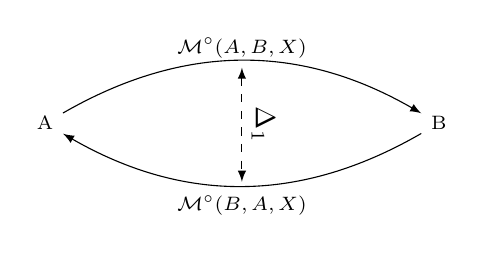
\begin{tikzpicture}[>=latex, scale=0.5]

\draw(0,0) node[anchor=north] (A) {\scriptsize A};
\draw(10,0) node[anchor=north] (B) {\scriptsize B};
\draw(5,2) node[anchor=north] {\scriptsize \Model{A}{ B}{ X}};
\draw(5,-2) node[anchor=north] {\scriptsize \Model{B}{ A}{ X}};
\draw[dashed, <->] (5,1) -- (5,-1.9) node[midway, sloped, above] {$\Delta_1$};
\draw[->] (A) to[bend left] (B);
\draw[->] (B) to[bend left] (A);

\end{tikzpicture}

\caption{\small Mutual modelling in a dyadic interaction, $\Delta_1 =
    \Delta(\mathcal{M}^{\circ} (A,B,X),
\mathcal{M}^{\circ} (B,A,X))$}

\label{mm_symmetry}
\end{figure}

\paragraph{The triangle questions}

With triads, we may compute the accuracy of 6 models:
\Model{A}{B}{X}, \Model{B}{A}{X}, \Model{A}{C}{X}, \Model{C}{A}{X},
\Model{C}{B}{X} and \Model{B}{C}{X}.

This leads to two \emph{triangle questions} (Fig.~\ref{mm_triangles}): Do $A$
and $B$ have the same accuracy when modelling $C$ ($\Delta_2 =
\Delta(\mathcal{M}^{\circ}(A,C,X), \mathcal{M}^{\circ}(B,C,X))$)? If it is the
same, $\mathcal{H}_{2}$ and $\mathcal{H}_{3}$ gains over $\mathcal{H}_{1}$

Conversely, does $C$ model more accurately $A$ than $B$ ($\Delta_3=
\Delta(\mathcal{M}^{\circ}(C,A,X), \mathcal{M}^{\circ}(C,B,X))$)? A positive
answer would support $\mathcal{H}_{3}$. A negative answer would support
$\mathcal{H}_{2}$ since $\Delta_3$ could mainly be explained by the way $A$ and
$B$ help $C$ to model them.

\begin{figure}[htb]
\centering
\subcaptionbox{}{ 
    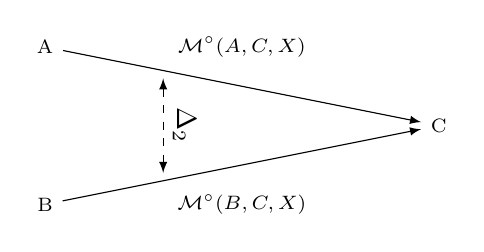
\begin{tikzpicture}[>=latex, scale=0.5]

    \draw(0,2) node (A) {\scriptsize A};
    \draw(0,-2) node (B) {\scriptsize B};
    \draw(10,0) node (C) {\scriptsize C};

    \draw(5,2) node {\scriptsize \Model{A}{ C}{ X}};
    \draw(5,-2) node {\scriptsize \Model{B}{ C}{ X}};
    \draw[dashed, <->] (3,1.2) -- (3,-1.2) node[midway, sloped, above] {$\Delta_2$};
    \draw[->] (A) to (C);
    \draw[->] (B) to (C);

    \end{tikzpicture}
}
\subcaptionbox{}{ 
    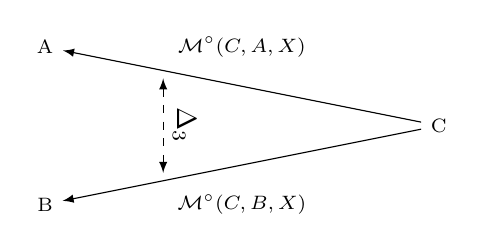
\begin{tikzpicture}[>=latex, scale=0.5]

    \draw(0,2) node (A) {\scriptsize A};
    \draw(0,-2) node (B) {\scriptsize B};
    \draw(10,0) node (C) {\scriptsize C};

    \draw(5,2) node {\scriptsize \Model{C}{ A}{ X}};
    \draw(5,-2) node {\scriptsize \Model{C}{ B}{ X}};
    \draw[dashed, <->] (3,1.2) -- (3,-1.2) node[midway, sloped, above]
    {$\Delta_3$};
    \draw[<-] (A) to (C);
    \draw[<-] (B) to (C);

    \end{tikzpicture}
}
\caption{\small Mutual modelling in a triadic interaction}

\label{mm_triangles}
\end{figure}



In addition, the comparison between $\Delta_2$ and $\Delta_3$ could tell us
whether the accuracy of mutual modelling depends more upon the modeller's effort
or the modellee's behaviour.

\paragraph{The rectangle questions}

We can go further by comparing self- versus other modelling ($\Delta_4$ in
Fig.~\ref{mm_rectangle}) as an indication of meta-cognitive skills. We can also
question if modelling skills depend upon what aspects are being modeled ($X$ or
$Y$), which would explain vertical differences ($\Delta_5$ in
Fig.~\ref{mm_rectangle}). When possible, we will also discuss these two
questions in the studies presented hereafter.

\begin{figure}[htb]
\centering

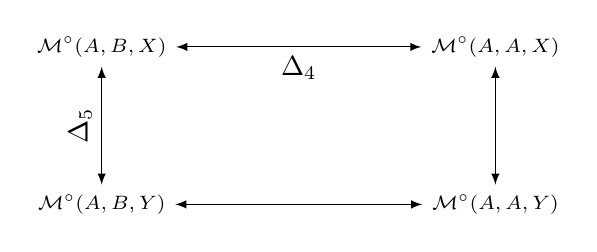
\begin{tikzpicture}[>=latex, scale=0.5]

    \draw(0,0) node (a) {\scriptsize \Model{A}{ B}{ X}};
    \draw(10,0) node (b) {\scriptsize \Model{A}{ A}{ X}};
    \draw(10,-4) node (c) {\scriptsize \Model{A}{ A}{ Y}};
    \draw(0,-4) node (d) {\scriptsize \Model{A}{ B}{ Y}};
    \draw[<->] (a) -- (b) node[midway, below] {$\Delta_4$};
    \draw[<->] (b) -- (c);
    \draw[<->] (c) -- (d);
    \draw[<->] (d) -- (a) node[midway, sloped, above] {$\Delta_5$};

\end{tikzpicture}

\caption{\small Meta-cognitive skills and domain-dependent modelling}

\label{mm_rectangle}
\end{figure}


This simple notation does not pretend to provide a mathematical account of
mutual modelling but to be more systematic in describing the following
experiments. 


%%%%%%%%%%%%%%%%%%%%%%%%%%%%%%%%%%%%%%%%%%%%%%%%%%%%%%%%%%%%%%%%%%%%%%%%%%%%%%%%%%
%%%%%%%%%%%%%%%%%%%%%%%%%%%%%%%%%%%%%%%%%%%%%%%%%%%%%%%%%%%%%%%%%%%%%%%%%%%%%%%%%%

\section{Studies}



%%%%%%%%%%%%%%%%%%%%%%%%%%%%%%%%%%%%%%%%%%%%%%%%%%%%%%%%%%%%%%%%%%%%%%%%%%%%%%%%%%
\subsection{{\bf Study 1}: Effect of an awareness tool on \gModel{A}{B} in a virtual
game}

We studied the impact of an awareness tool on group performance and mutual
modelling~\citep{nova2007collaboration}. The availability
of an awareness tool was our independent variable. In previous studies, we
replayed a video of the game to subjects who surprised us by their ability to
remember former states of their mutual model: ``I did that because I thought that
you would do that''. Hence, this experiment focused the representation of each
other's action plans. During the game, we asked them to anticipate the next
action of their partner as well as to announce their own actions.

\subsubsection*{Experimental setting}

\begin{figure*}
        \centering
        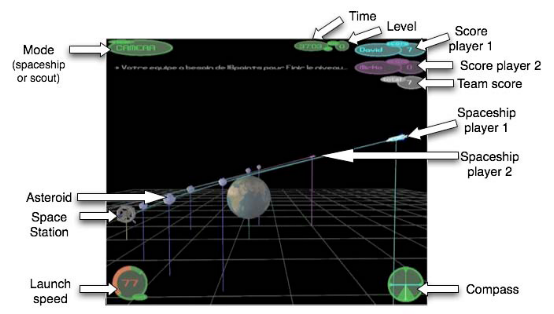
\includegraphics[width=\textwidth]{image4.png}
        \caption{Screenshot of the {\sc SpaceMiners} game}
        \label{study1:spaceminer}
\end{figure*}


{\sc SpaceMiners} is a 3D game that involves two players collecting minerals located
in asteroids (Fig.~\ref{study1:spaceminer}). To do so, they must launch drones through
the space after choosing their initial direction and speed. Once launched, the
trajectory of drones is only influenced by the gravity of planets and by
trajectory modification tools.  During the experiment, the teams were confronted
with three increasingly complex situations. The experiment was 2 hours long: a
30 minutes tutorial and 3 levels of 30 minutes. Players uses using a regular
joystick and communicated with each other through an audio channel.

The independent variable was the availability of an awareness tool that shows to
player $A$  the location and gaze direction of player $B$. In the awareness
condition, players could switch to the \emph{scout mode} where they could view what
their partner was looking at. We hypothesize that this would enable subjects to
more accurately infer their teammate's intentions. Each player sat in front of a
distinct computer located in different rooms. 

\subsubsection*{Subjects}

Thirty-six persons participated in this study, all native French speakers. We
constituted 18 dyads who did not know each other beforehand. The pairs were
randomly assigned to either the control condition (without the awareness tool)
or the awareness condition (with the awareness tool).

\subsubsection*{Variables}

Task performance was measured by the score reached by the two subjects at the
end of the game (three levels). The effort of mutual modelling was measured as
the ratio of time that players would spend in the scout mode (divided by total
time), which is the time during which players are not performing their own
actions but monitoring their partner's actions.

In order to evaluate \gModel{A}{B} during the task, we used two questionnaires
(Fig.~\ref{study1:questionnaires}) that were displayed during each of the three
games, as a transparent layer appearing over the game display. The first
questionnaire concerned the player's intended actions. The second questionnaire
asked each player about what he thought her or his partner was intending to do.
Some answers were identical in both questionnaires (like ``adjusting a shot'')
while others were reversed (``to guide my partner'' versus ``to guide me'').
This method provides us with a subjective measure of accuracy
($\Delta(\M{A}{A}{X}, \M{A}{B}{X})$) rather than an objective measure (\ie the
model \gmodel{A}{B} is compared to $B$'s next action) because some of the
activities proposed by the questionnaire were not observable by the environment
(\eg establishing a strategy). We calculated \Model{A}{B}{activity})
as the number of common answers between questionnaires \gmodel{A}{A} and
\gmodel{A}{B} in each game and computed the average value a across the 3 levels.

\begin{figure}[ht!]
        \centering
        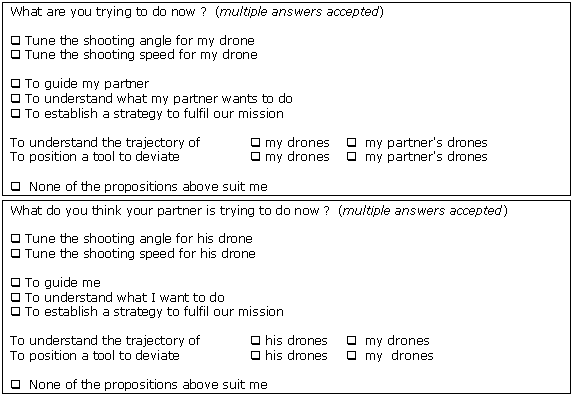
\includegraphics[width=0.7\columnwidth]{image5.png}
        \caption{\gmodel{A}{A} and \gmodel{A}{B} questionnaires in SpaceMiners
        (translated from French).}

        \label{study1:questionnaires}
\end{figure}

\subsubsection*{Results}

\paragraph{Grounding criterion} The grounding criterion was high: the
correlation between \gModel{A}{B} and task performance was 0.42, $p = 0.05$.
Pairs with an accurate mutual model reached higher scores. A regression analysis
confirmed the positive and significant relation between group performance and
mutual modelling accuracy ($\beta=54, p = 0.02$).

\paragraph{Study-specific questions} The awareness tool permitted higher group
performance, but it did not improve the accuracy of the mutual model. Since
teams were free to use the awareness tool or not (the \emph{scout} mode), we
performed a post-hoc split of players depending on how much time they used it.
The split point was the mean of time spent in the scout mode and it led to the
constitution of two groups made up of 12 individuals ``short time in scout
mode'' and 24 individuals ``long time in scout mode''. A two-way analysis of
variance conducted on these contrasted groups revealed that pairs in the
awareness condition who spent more time in the scout mode reached higher levels
of \gModel{A}{B}($F = 8.02, p = 0.015$). Of course, a \textit{post-hoc} split
does not support a causal direction. An alternative explanation could be that
good modellers are more social and hence appreciate the awareness tool.

\paragraph{Symmetry question} We computed intra-class correlation as described
by~\citet{kenny1998data} from the answers to the cross-questionnaires.
Considering all pairs in both conditions, we found a positive and significant
correlation ($r = 0.38, p < 0.05$) between \gModel{A}{B} and \gModel{B}{A}.
Interestingly, this was higher in the control group ($r = 0.44$) than in the
experimental group ($r = 0.24$). Actually, $\Delta(\gMdeg{A}{B},\gMdeg{B}{A})$,
\ie the absolute differences between the models accuracy, was not significantly
different with or without the awareness tool ($F [1,13]= 0.144, p > 0.5$). This
result could be explained by the fact that the players without awareness tools
communicated more.

\subsubsection*{The triangle and rectangle questions are not addressed in this study.}

\subsubsection*{Discussion}

How to interpret a correlation of 0.38 between \gModel{A}{B} and \gModel{B}{A}?
If it was null, modelling would be interpreted as an individual process that
varies according to personality traits or cognitive skills: some persons tend to
model more accurately their peer while others don't care or can simply not
($\mathcal{H}_{1}$). If the correlation was close to 1, we could conclude that
the modelling accuracy is an emergent property of teams since there would be low
probability that, by chance, low accurate modellers are paired with accurate
modellers and conversely ($\mathcal{H}_{2}$). Our correlation is between these
two extremes but the very notion of significant intra-class correlation tend to
indicate that one may not consider peers as independent subjects, which is an
argument for the \emph{interaction} hypothesis $\mathcal{H}_{3}$. 


%%%%%%%%%%%%%%%%%%%%%%%%%%%%%%%%%%%%%%%%%%%%%%%%%%%%%%%%%%%%%%%%%%%%%%%%%%%%%%%%%%
\subsection{{\bf Study 2}: Effect of an awareness tool on \gModel{A}{B}  in a pervasive
game}

This study concerns a collaborative game that occurred in the physical
space~\citep{nova2006underwhelming}. We studied whether players build an accurate
model of the path followed by their partners, assuming this path reflected their
problem solving strategy. We used an objective measure of \gModel{A}{B}: the
distance between where $A$ believes $B$ has been walking and where $B$ actually went.
The main hypothesis concerned the effect of awareness tools on group performance
and on \gModel{A}{B}. 

\subsubsection*{Experimental setting}

{\sc CatchBob} is a mobile game in which groups of 3 players have to solve a
joint task. The game was played on EPFL campus. Participants had to find a
virtual object (\emph{Bob}) and to ``catch'' it by forming a triangle around it.
Players used a Tablet PC that displayed a map of the campus and an indication of
their personal distance to Bob. Their annotations on the map were shared with
the two other players ($A$ could see what $B$ and $C$ wrote). These annotations
faded out after a few minutes to avoid covering the full display. The awareness
tool displayed as well the location of the two other players on the map. This
resulted in three conditions: the control condition (without tool) and two
experimental conditions: synchronous awareness (display of the current position
of each player) and asynchronous awareness (display of current position of each
player as well as their recent spatial trace).

\begin{figure*}[h!t]
        \centering
        \begin{subfigure}{.45\textwidth}
            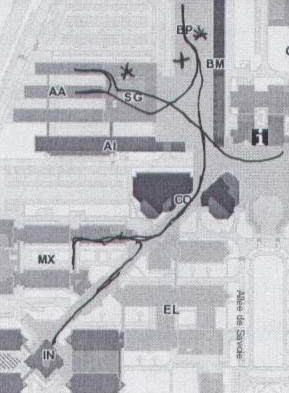
\includegraphics[width=\linewidth]{image6.png}
            \caption{A's drawing of $B$'s path.}
        \end{subfigure}
        \begin{subfigure}{.4\textwidth}
            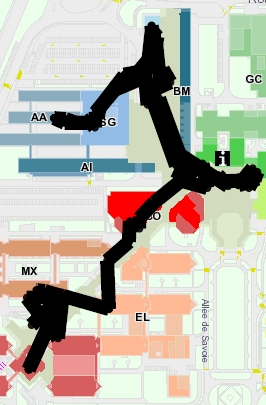
\includegraphics[width=\linewidth]{image7.png}
            \caption{Actual path followed by $B$.}
        \end{subfigure}
        \caption{Reported and actual path of one of the player, during the {\sc
        CatchBob} game.}
        \label{study2:paths}
\end{figure*}

\subsubsection*{Subjects}

Ninety EPFL students participated in this experiment. We only selected EPFL
students since knowledge of the campus geography had an impact both on group
performance and on mutual modelling: to represent the path of someone across
some space is difficult without an \textit{a priori} mental map of this space.
We formed groups of students who knew each other. We assigned 10 triads to each
of our three experimental conditions. Each condition was made up of
approximately 25\% of women, but we did not control gender repartition within
each triad.

\subsubsection*{Variables}

The independent variable was the presence and role of the awareness tool. As a
dependent variable, we had the task performance which was the distance covered
by the team to catch Bob and \gModel{A}{B}. To estimate \gModel{A}{B}, we asked
players to draw on paper their own path and the path of each of their partners
after the game. This enabled us to calculate the number of errors players made
while drawing the path of their partners. We compared the path that player $A$
attributed to $B$ with $B$'s real path recorded by the system and the same for
$A$ \& $C$ and $B$ \& $C$ as depicted on Fig.~\ref{study2:paths}. 

\gModel{A}{B} is the sum of errors made by $A$ about $B$'s paths. An error was
either drawing a place where the partner had not been or not drawing a place
where he/she had gone. One could argue that \gModel{A}{B} is biased by the
subjects' ability to translate their trajectories souvenir into a map drawing.
However, 85\% of subjects made no mistake at all when drawing their own path. We
therefore consider mistakes in their partners' path as being due to a lack of
mutual modelling accuracy instead of being due to spatial reasoning skills.

\subsubsection*{Results}

\paragraph{Grounding criterion} The correlation between \gModel{A}{B} and the
task performance (path lengths) was low: 0.15. Using a \emph{post-hoc} split on
\gModel{A}{B}, there is no significant difference between the performance of the
groups with high and low \gModel{A}{B}  ($F = 1.45, p = 0.24$). Conversely, a
\emph{post-hoc} split of the groups according to their performance did not show
any significant differences on \gModel{A}{B} ($F = 1.16, p = 0.29$).

\paragraph{Study-specific questions} There was no significant difference
regarding the task performance. However, and surprisingly, the absence of the
awareness tool was related to a higher \gModel{A}{B}: players tended to better
remember their partners' paths when they could not constantly monitor their
positions. As detailed in the original study~\citep{nova2005location}, it
appeared that teams without awareness tool made more manual annotations on the
map while permanent monitoring has an underwhelming effect.

\paragraph{Symmetry question} The correlation between \gModel{A}{B}  and
\gModel{B}{A}  is positive ($r = 0.41$) and significant ($p < 0.01$): the more $A$
makes errors about $B$, the more $B$ does as well.

\paragraph{Triangle questions} Regarding $\Delta_2$, the correlation between
\gModel{A}{C} and \gModel{B}{C} is significant: $r=0.43, p <.001$. Concerning
$\Delta_3$, the correlation between \gModel{A}{B} and \gModel{A}{C} is
significant as well: $r=0.30, p <.01$.

\subsubsection*{Discussion}

This positive correlation observed in the symmetry question is surprising as
well: when acknowledging the high heterogeneity of spatial skills among
adults~\citep{liben1981spatial}, a significant positive correlation would
indicate that mutual modelling indeed stems from group processes more than
individual processes. The significant results on the triangle questions goes in
the same direction: either both the modeler and the modellee contribute to
accurate modelling, or the quality of teamwork has a global effect. Since team
members did not have many opportunities to directly interact during this
experiment, the factor that facilitates accurate mutual modelling is probably
more the overall group strategy than the quality of verbal interactions: a clear
strategy facilitates memorizing one's partner path. 




%%%%%%%%%%%%%%%%%%%%%%%%%%%%%%%%%%%%%%%%%%%%%%%%%%%%%%%%%%%%%%%%%%%%%%%%%%%%%%%%%%
\subsection{{\bf Study 3}:  Effect of media richness on \gModel{A}{B} in argumentation}

The aim of this unpublished\footnote{The data and statistical analyses of this
study are available online:
\url{https://github.com/chili-epfl/mutual-modelling-emotions-study}.}
study was to evaluate the effect of media richness on \Model{A}{B}{emotions}.
The hypothesis was that video communication would lead to a better \gModel{A}{B}
than audio only since emotions often impact on facial expressions.

\begin{figure*}[ht!]
        \centering
        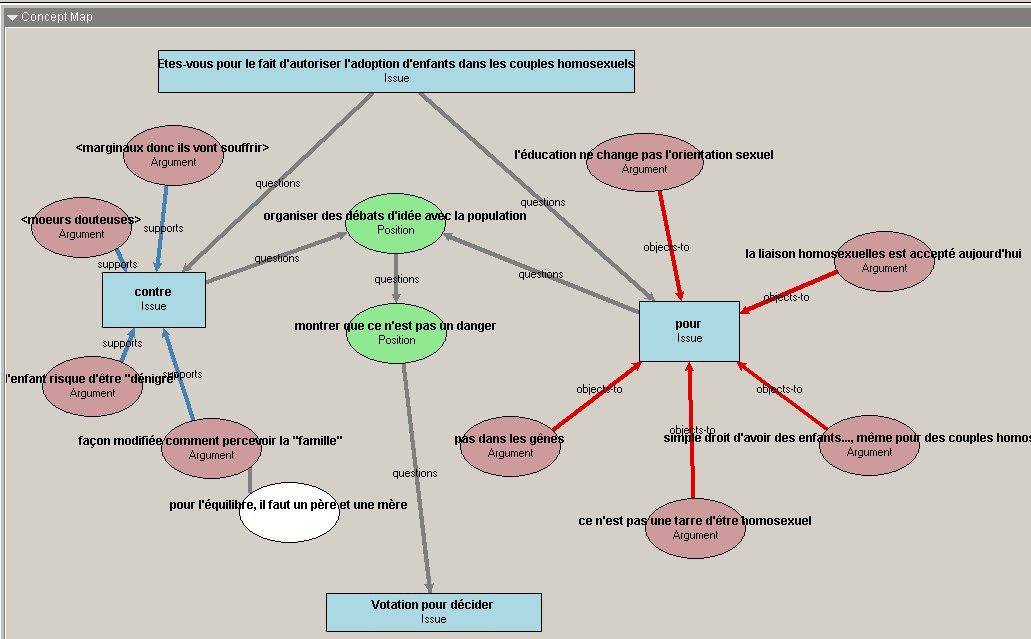
\includegraphics[width=\textwidth]{image8.jpg}
        \caption{Example of argumentation graph}
        \label{study3:argumentation_graph}
\end{figure*}


\subsubsection*{Experimental settings} 

Triads had to address an emotional societal debate: authorizing or not adoption
by homosexual couples. They worked on-line and had to structure their
argumentation with the shared concept map tool {\sc TeamWave} as illustrated in
Fig.~\ref{study3:argumentation_graph}. Ten groups had only an audio connection
while ten groups had audio and video. The video communication was provided by a
webcam and the software {\sc IVisit}. For the audio link, we used microphones,
headsets and the {\sc BattleCom} software. In the \emph{audio plus video}
condition, the screen was divided in three sections. The main part was devoted
to the concept map window, and the images of the two peers appeared next to it.
In the audio condition, this video zone was left empty so that the size of the
concept map was equal in each condition. The subjects were located in the same
room, separated by mobile walls. Despite their headsets, non-verbal audio cues
(\eg tapping the floor with feet) were possibly heard by the participants. The
task lasted in average 61 minutes.

\subsubsection*{Subjects}

Sixty students (twenty triads) from the University of Geneva participated to
this experiment (36 women and 24 men). We formed groups of subjects who knew
each other: the task required the discussion of sensitive issues which required
to feel quite comfortable with peers. Since groups were formed \textit{a
priori}, we did not balance gender in each condition.

\subsubsection*{Variables}

The independent variable was the presence or not of a video link. The dependent
variable \gModel{A}{B} was measured subjectively from three questionnaires: in
the first one, $A$ described his/her own emotions \gmodel{A}{A}, while in the
two other questionnaire, $A$ described $B$'s and $C$'s emotions. The questionnaire
included 18 items (7-point Likert Scale) describing emotions labeled as
adjectives: \emph{anxious}, \emph{enthusiastic}, \emph{agitated}, \emph{proud},
\emph{excited}, \emph{quiet}, \emph{calm}, \emph{stressed}, \emph{bored},
\emph{upset}, \emph{relaxed}, \emph{irritated}, \emph{determined},
\emph{hostile}, \emph{active}, etc. \gmodel{A}{B} was modelled as a vector of 18
numerical values corresponding to their answers on each questionnaire items, and
\gModel{A}{B} was computed as the distance between the two vectors
\gmodel{A}{B} and \gmodel{B}{B}:

\[
    \Mdeg{A}{B}{emotions} = \frac{\displaystyle\sum_{emotions} \abs{\M{A}{B}{e} -
    \M{B}{B}{e}}}{18}
\]

The smaller the score, the \emph{more} accurate the model.

\subsubsection*{Results}

\paragraph{Grounding criterion} The maps produced by teams were ranked by three
independent judges on completeness and structure quality (Kendall's $W=0.474$,
limited agreement). We used the average rank as a estimation of the team
performance and correlated it with the average of the 6 values of \gModel{A}{B}
per team (\gModel{A}{B}, \gModel{A}{C}, \gModel{B}{A},...). The correlation is
0.22: teams with a good \gModel{A}{B} tend to be better ranked. 

\paragraph{Study-specific questions} Our hypothesis about media richness is
rejected: the average score for \model{A}{B}{emotions} was 1.25 ($SD = 0.53$) in
the audio+video condition and 1.09 ($SD = 0.41$) in the audio alone condition
($t=1.89, df=111, p = 0.062$): the average degree of accuracy of
\model{A}{B}{emotions} was hence \emph{higher} in the audio alone condition.

\paragraph{Symmetry question} We computed the absolute differences $\Delta_1$
between \gModel{A}{B} and \gModel{B}{A} over all pair of subjects within a triad
(3 values per triad, 20 triads), and compared them with the same differences
computed from random gradings (following the same grade distribution as for the
experimental data).

A t-test on the two sets releaved a significantly lower average difference in
the experimental data (mean difference: $0.40$ vs $0.54$ with random gradings,
$t=-3.3, df=60, p = 0.0016$), supporting $\mathcal{H}_{2}$ or $\mathcal{H}_{3}$.

\paragraph{Triangle questions} $\Delta_2$ is computed in a similar way as the average of
the absolute differences between \gModel{A}{C} and \gModel{B}{C} over the 60
subjects. The average difference is 0.42 ($SD= 0.34$), and if not significantly
different from the same data obtained from random gradings ($t=-1.61, df=60,
p=0.11$). This rejects $\mathcal{H}_{2}$.

For $\Delta_3$, the average absolute difference between \gModel{C}{A} and
\gModel{C}{B} over the 60 subjects is 0.40 ($SD= 0.41$) and is significantly
lower than chance ($t=-2.62, df=60, p=0.01$): a given subject tends to model its
two partners with similar degrees of accuracy, which supports $\mathcal{H}_{1}$.
It could also support $\mathcal{H}_{3}$, but it does not since $\Delta_2$ is not
significant.

\begin{figure*}[ht!]
        \centering
        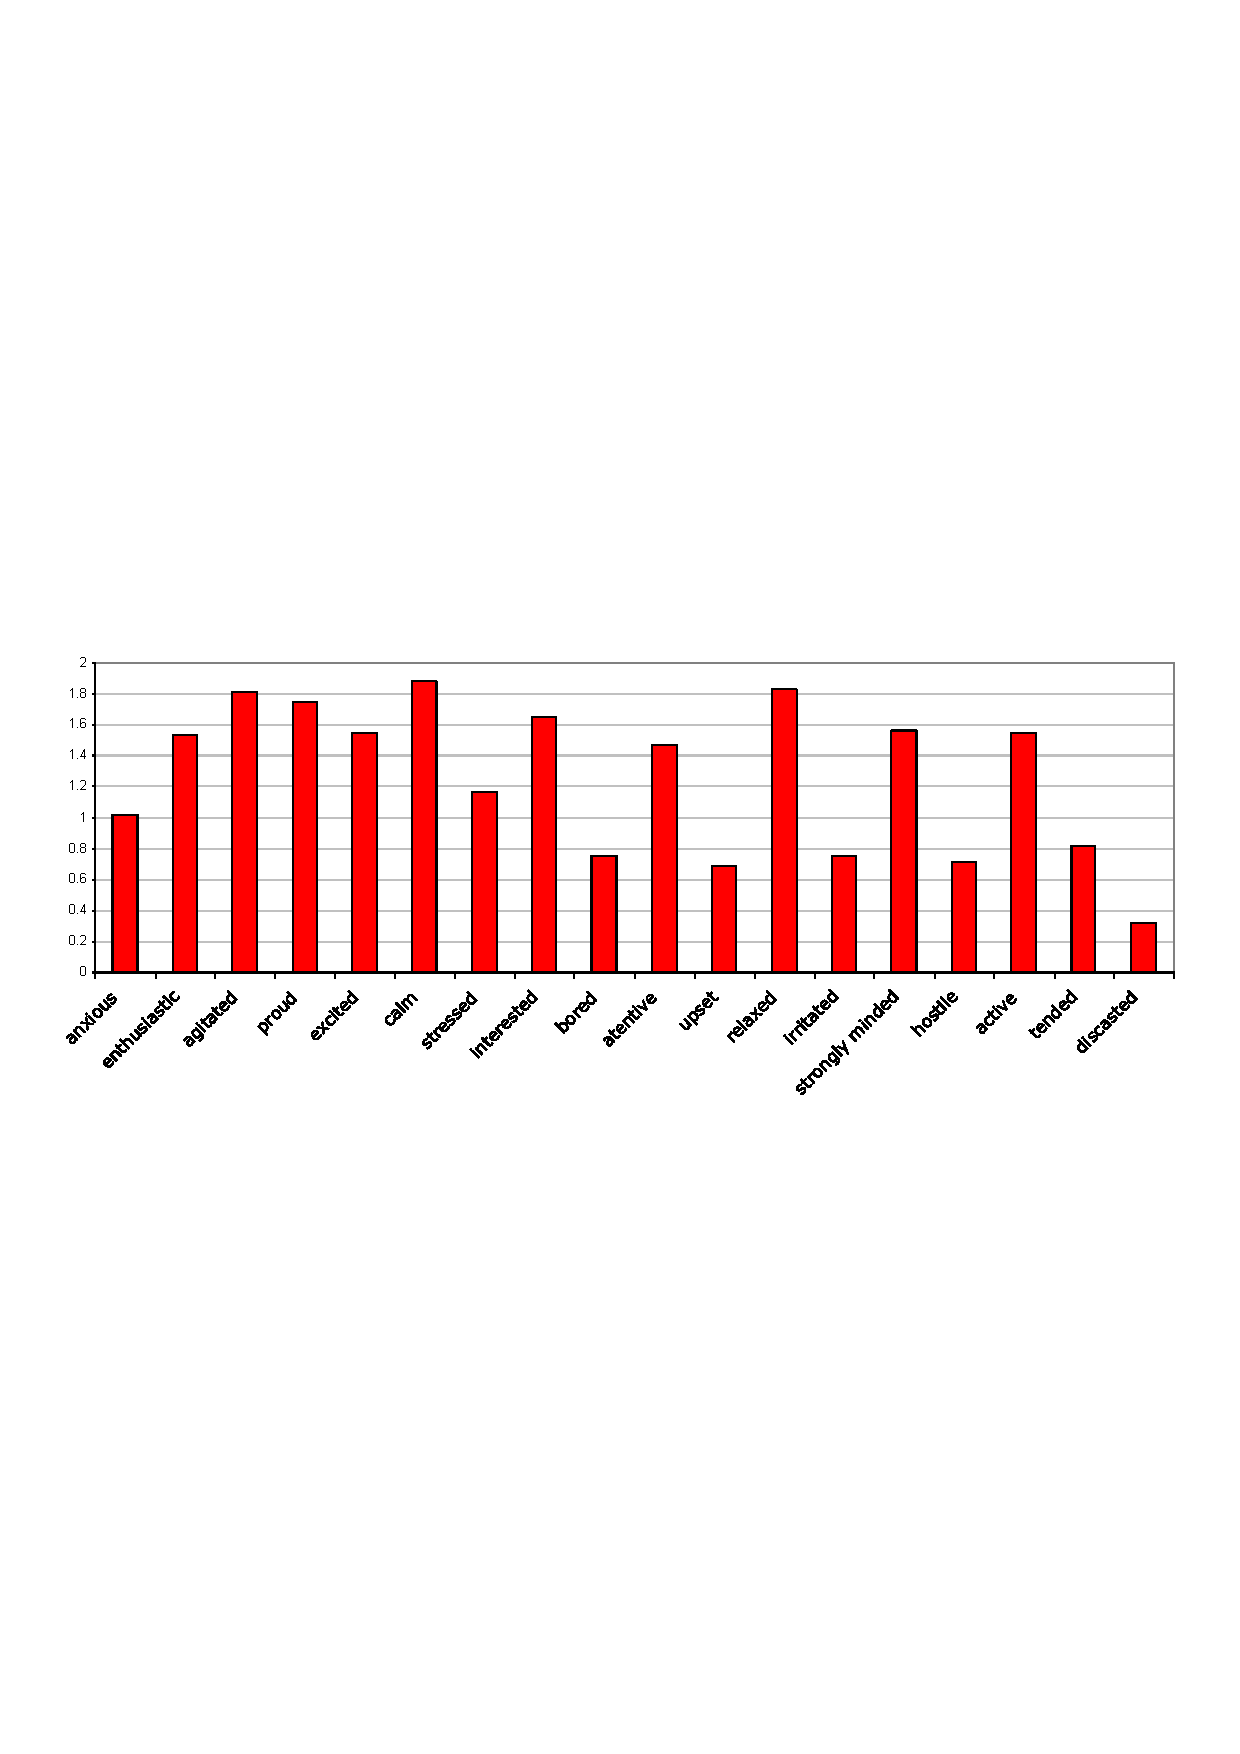
\includegraphics[width=\textwidth]{image9.pdf}
        \caption{Average values of \Model{A}{B}{X} where $X$ is one of the proposed
        emotions (max = 7).}
        \label{study3:deg_m_values}
\end{figure*}


\paragraph{Rectangle question} We cannot address the relationship ($\Delta_4$)
between self and social accuracy here because we do not have an estimation of
self-accuracy: subjects describe their emotions but we have no way to check if
there are correct. By measuring \gModel{A}{B} on  18 emotional labels,
we can however have a glimpse about $\Delta_5$: how \Model{A}{B}{X} varies
according to X.  Fig.~\ref{study3:deg_m_values} shows the range of modelling
errors: the difference between \gmodel{A}{B} and \gmodel{B}{B}, on a scale of 7,
is 0.3 in average for the emotion \emph{discasted}, and up to 1.9 for the
emotion \emph{calm}. This is probably specific to the variety of scales  ($SD=
0.5$ for \emph{discated} versus $SD=0.7$ for \emph{calm}), our point is not to
interpret this too far, but to show that there are large variations even within one
area  (perceiving emotions).

\subsubsection*{Discussion}

The results evidence that richer media does not automatically foster better
modelling, on the contrary: groups using only the audio modality to exchange
their views were able to build more accurate models of each others than groups
using both video and audio, which is especially surprising when modelling
emotions: one would expect that video feedback indeed help building a better
model of the emotions of the other. Our interpretation is that viewing what
one's partner sees (shared graphical editor) was, in this task, more important
than seeing each other~\citep{gaver1993one,anderson1997impact}.

In this study, the accuracy of mutual modelling between two peers tend to be
symmetrical, which would support the idea that the quality of modelling is primarily
building upon the social interaction. This is however not fully supported by the
analysis of $\Delta_2$: $A$ being good at modelling $C$ does not correlate with
$B$ being good at modelling $C$.

On the other hand, $\Delta_3$ shows that a given $A$ tends to
model $B$ and $C$ at similar levels of accuracy: this evidences an individual
skill at modelling others (hypothesis $\mathcal{H}_{1}$).


%%%%%%%%%%%%%%%%%%%%%%%%%%%%%%%%%%%%%%%%%%%%%%%%%%%%%%%%%%%%%%%%%%%%%%%%%%%%%%%%%%
\subsection{{\bf Study 4}:  Effects of a script on \gModel{A}{B}  in concept mapping}

This study investigated the effect of a collaboration script on collaborative
learning~\citep{molinari2008effects}. The script chosen is a {\sc jigsaw}: two students
receive different but complementary subsets of the knowledge (texts) which have
to be integrated to build a shared concept map.  This script increases the
cognitive effort to build the map, not only to conciliate the viewpoints of
each team members but, before that, to find out what the other knows. 

\subsubsection*{Experimental settings}

The instructional material consisted of an explanatory text about the
neurophysiologic phenomenon of \emph{action potential}. The text was divided
into 3 chapters.  In the \emph{same information} (SI) condition, the same text
was given to both partners. In the \emph{complementary information} (CI)
condition, it was divided into two sub-texts, one about the electrical processes
of the neuron while the second one about the chemical processes. These two
versions were equivalent in terms of number of information pieces. 

The peers were located in two rooms equipped with the same
computer.  The experimental session lasted around 90 minutes and consisted of 6
phases: Participants used two software components, {\sc CmapTools} and {\sc
TeamSpeak}.

\begin{enumerate}

    \item As a pre-test, participants were asked to write down all they knew
        about the neuron and its functioning (5 minutes),

    \item Participants were instructed to read a text (12 minutes),

    \item Participants were asked to build individually a concept map in order to
        graphically represent what they learnt from the text (10 minutes),

    \item Dyads had to built a concept map during 20 minutes, communicating by
        audio.  The screen layout was structured into three areas
        (Fig.~\ref{study4:concept_map}),

    \item Participants were invited to individually complete a knowledge test
        (15-20 minutes),

    \item Participants where asked to estimate their own- and their partner's
        final knowledge in a questionnaire. 

\end{enumerate}



\begin{figure*}
    \centering
    \begin{tikzpicture}[scale=1]
        \node[anchor=south west,inner sep=0] at (0,0)
            {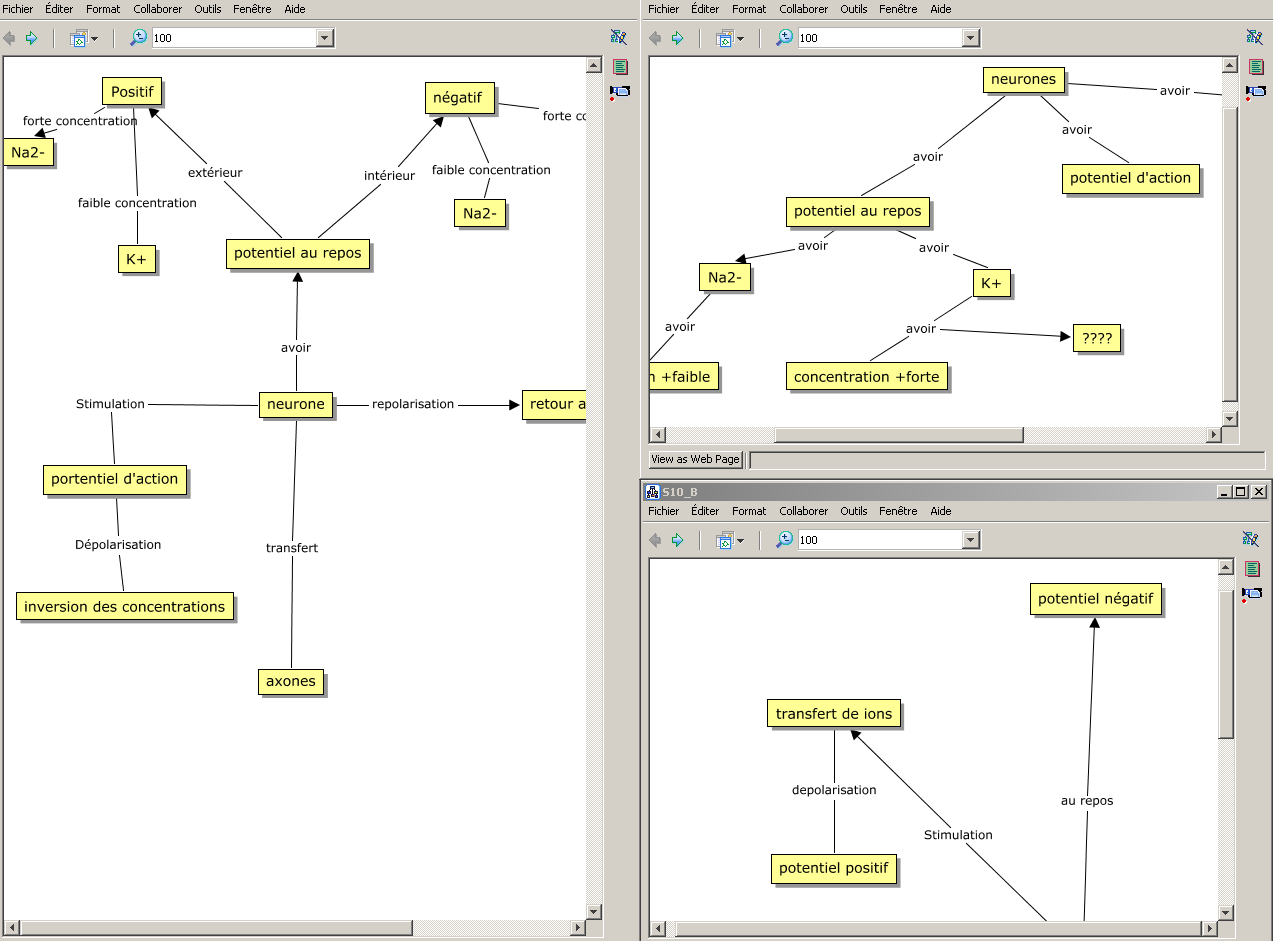
\includegraphics[width=0.75\textwidth]{image10.png}};
        
            \node[rectangle,draw, thick] at (8,4.3) {Self map};
            \node[rectangle,draw, thick] at (6,2.6) {Partner map};
            \node[rectangle,draw, thick] at (2.5,1.5) {Collaborative map};
    \end{tikzpicture}
    \caption{The group concept map and the individual concept maps in study
    4}
    \label{study4:concept_map}
\end{figure*}

\subsubsection*{Subjects}

Fifty-eight first year students from EPFL (47 men and 11 women, mean age: 20.46)
were remunerated for participation. Dyads were randomly assigned to one of the
two experimental conditions. Gender was balanced over the conditions.
Participants did not know each other before the experiment. Students from Life
Sciences faculty were not recruited to avoid high initial background knowledge on the
learning domain.

\subsubsection*{Variables}

The independent variable, script versus no-script, was implemented by the
difference of texts that individuals had to read.  The dependent variables were
the post-test scores, used to assess \Model{A}{B}{knowledge}. In phase 6,
participants were ask to estimate (7-point Likert scale) their own and their
partner's outcome knowledge with respect to each chapter of the learning
material. The order of questions about oneself and about the other was
counterbalanced across participants. 
%We measure \gModel{A}{B} in an objective
%(Eq.~\ref{eq:study4.1} and \ref{eq:study4.2}) as well as in a subjective way
%(Eq.~\ref{eq:study4.3}).
%
%\begin{multline} \label{eq:study4.1}
%    \Mdeg{A}{B}{knowledge} = 
%        \sum_{i=1}^{3} (\M{A}{B}{chapter_i} - score(B, chapter_i))
%\end{multline}
%
%\begin{multline} \label{eq:study4.2}
%    \Mdeg{A}{A}{knowledge} = 
%        \sum_{i=1}^{3}  (\M{A}{A}{chapter_i} - score(A, chapter_i))
%\end{multline}
%
%\begin{multline} \label{eq:study4.3}
%    \Mdeg{A}{B}{knowledge} = 
%        \sum_{i=1}^{3}  (\M{A}{B}{chapter_i} - \M{B}{A}{chapter_i})
%\end{multline}

\subsubsection*{Results}

\paragraph{Grounding criterion} In this task, the grounding criterion was low.
We did not however evaluate task performance (\eg the quality of the jointly
produced concept map) but learning gains. The correlation between \gModel{A}{B}
and $A$'s learning gains is not significant ($\beta = 0.08, ns, N = 60$). It is
also not significant within each condition.

\paragraph{Study-specific questions} We performed a non-parametric Mann-Whitney
test on post-test scores for electric questions and a one-way ANOVA on scores
for ionic questions (Levene tests for homogeneity of variances): $p = 0.02$ and
$ns$, respectively. Results  did not show any significant difference between the
\emph{same information} (SI) condition and the \emph{complementary information}
(CI) condition, neither for electric questions ($U = 388.50, z = -0.88, ns$) nor
for ionic questions ($F(1, 58) = 0.17, ns$).  The effect of scripts on
\gModel{A}{B} was not significant ($F(1, 58) = 0.78, ns$) when considering the
absolute difference between \gModel{A}{B} and $B$'s post-test score. However, $A$
tended underestimate $B$'s score in the SI condition ($M = -2.06$) and to
overestimate it in the CI condition ($M = 1.21$) ($F(1, 58) = 6.44, p<0.01$).
Regarding to \gModel{A}{A}, there was no significant difference between
conditions.

\paragraph{Symmetry question} The inter-class correlation between \gModel{A}{B}
and \gModel{B}{A} is approaching significance ($r= 0.26, F(1,29)=1.71, p=
0.075$). It is indeed significant when students read the same text (SI
condition: $r=0.43, F(1,15)=2.53, p<0.05$) but not when they read different texts
($r= 0.13, F(1,12)=1.3, ns$). 

\paragraph{Rectangle question} The correlation between \gmodel{A}{A}
and \gmodel{A}{B} ($\Delta_4$) is globally not significant ($r=0.05$) as well as not
significant in each condition: someone good at self-modelling is not necessarily
good at modelling someone else and vice-versa.

\subsubsection*{Discussion}

In this experiment, the symmetry of mutual modelling is only found when subjects
are in conditions of symmetry of information. This consolidates the hypothesis
of \gModel{A}{B} being a property of interactions in context ($\mathcal{H}_{3}$)
rather than $A$'s cognitive attitude.



%%%%%%%%%%%%%%%%%%%%%%%%%%%%%%%%%%%%%%%%%%%%%%%%%%%%%%%%%%%%%%%%%%%%%%%%%%%%%%%%%%
\subsection{{\bf Study 5}: \Model{A}{B}{knowledge} in concept mapping}

This study investigates if \Model{A}{B}{knowledge} is related to learning
outcomes by comparing teams with or without a knowledge awareness tool (KAT),
\ie a tool that informs $A$ about $B$'s knowledge as measured through a pre-test.

\subsubsection*{Experimental setting}

The peers were located into two different rooms. A complete description of the
study is provided in~\citet{sangin2008learners}. The experiment lasted 90 minutes.

It started with the same two first steps as in study 4, followed by:

\begin{enumerate}
    \setcounter{enumi}{2}

    \item Subjects passed a pre-test, with ten questions per chapter. 

    \item Participants had 20 minutes to draw a collaborative concept map
        reporting the content of the texts. They were able to communicate
        orally through headsets.  We used Tobbii eye tracking devices to
        record their gazes.

    \item The post-test included the same items than the pre-test but in a
        different order. 

    \item  Finally, participants were asked to estimate their partner's
        knowledge at the post-test for each of the three chapters on a 7-point
        Likert-like survey. 

\end{enumerate}

\begin{figure*}[h!t]
        \centering
        \begin{subfigure}{.6\textwidth}
            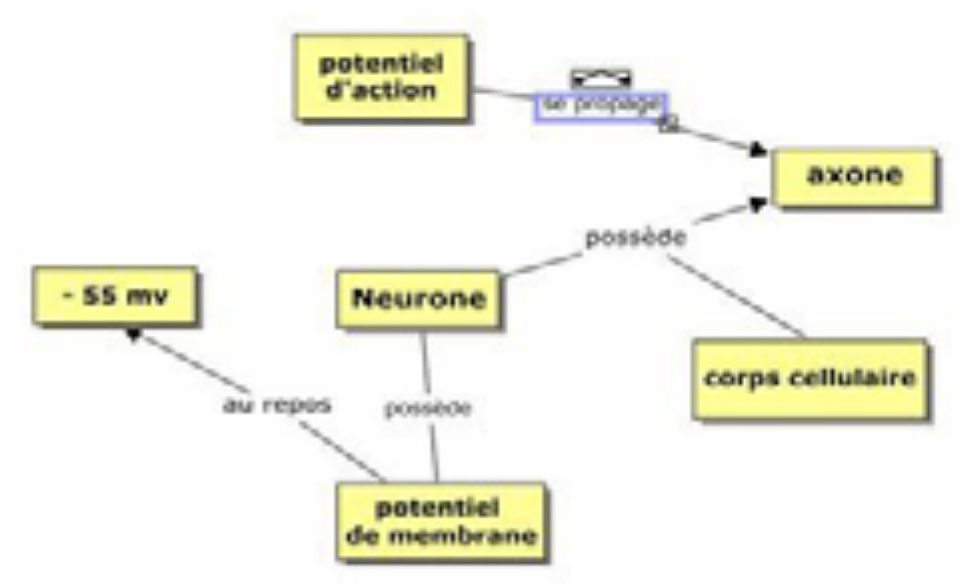
\includegraphics[width=\linewidth]{study5-conceptmap.png}
        \end{subfigure} \\
        \begin{subfigure}{.7\textwidth}
            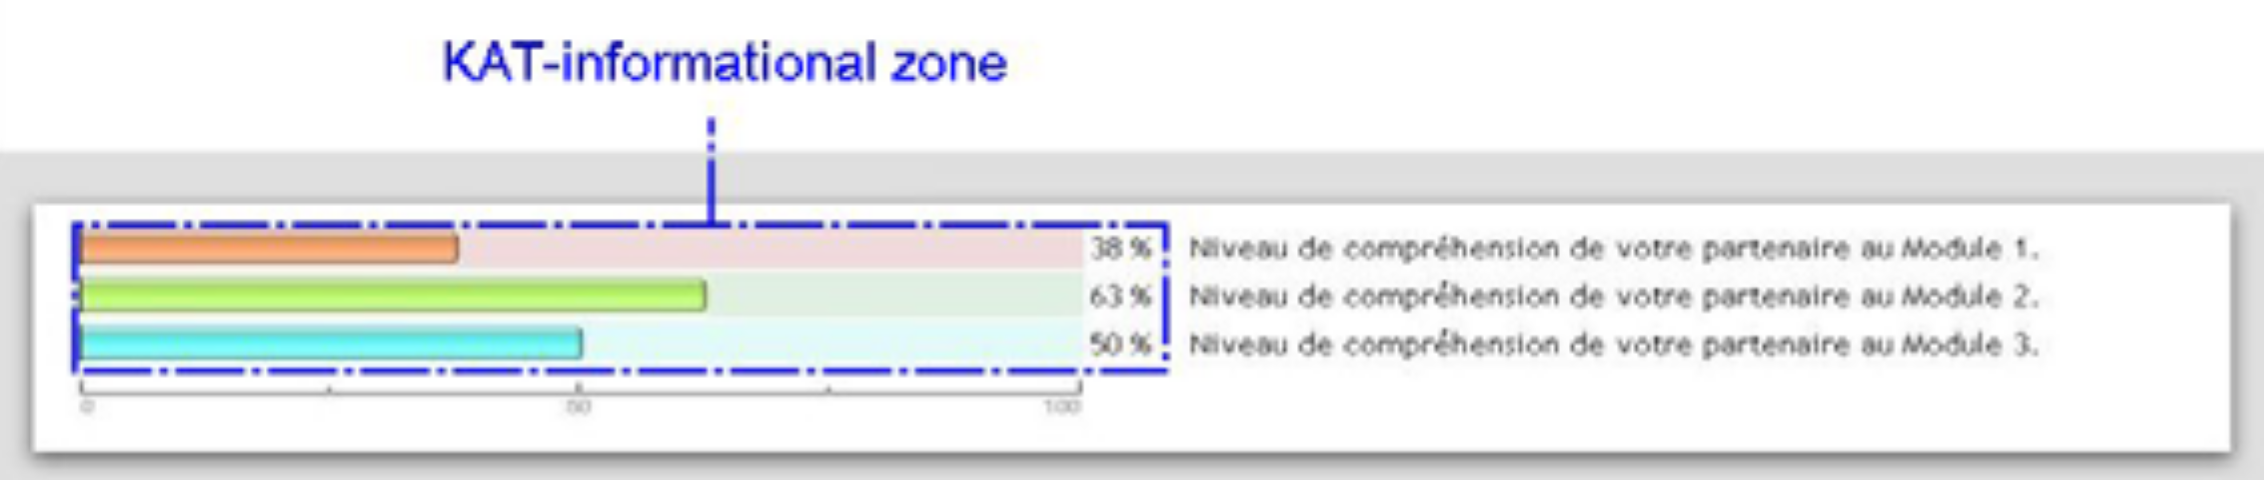
\includegraphics[width=\linewidth]{study5-kat.png}
        \end{subfigure}
        \caption{Screenshot of the KAT condition during the concept-map building
        phase.}
        \label{study5:kat}
\end{figure*}

\subsubsection*{Subjects}

Sixty-four first year EPFL students (46 men, 18 women, mean age: 21.2)
participated to the study. They were randomly assigned to conditions and
did not know each other before. Like in Study 4, students from Life Science
faculty were excluded.

\subsubsection*{Variables}

The participants of the experimental condition group were provided with the KAT
on the bottom part of the screen (Fig.~\ref{study5:kat}): each line represents
the score obtained by the partner at the pre-test for a chapter. Participants
did not see they own score, but they usually started their discussion by
exchanging this information.

\subsubsection*{Results}

\paragraph{Grounding criterion} A linear regression revealed a positive relation
between \gModel{A}{B} and the learning gain of the pair $\{A, B\}$ (calculated
as the average of the individual learning gains): $\beta= 0.401, p < 0.001, r2adj.
= 0.15$, large effect. This relationship was not significant in the previous
experiment which as been conducted with the same task (using the same task
should produce the same grounding criterion). This is probably due to the fact that
\gModel{A}{B} was influenced by the KAT.

\paragraph{Study-specific questions} The $t$-test reported a significant
difference between the KAT condition participants ($M = 13.4\%$) and the control
group [$M = 3.6\%, t(1, 60) = 2.73, p < 0.01$, Cohen's $d = 0.7$, medium to large
effect]: providing learners with cues about the prior-knowledge of their partner
enhances their collaborative learning. As a treatment check, we found a positive
and significant correlation between the amount of gazes on KAT (using eye
tracking devices) and the learning gains ($r(22) = 0.54, p = 0.01$). A detailed
analysis revealed that subjects look at KAT to assess their peer's credibility
when he/she provided new information. 

The KAT has a significant effect on \gModel{A}{B}: peers more accurately
estimated their partners knowledge ($M = 1.11$) than those in the control
condition [$M = 0.98, t(1, 60) = 3.19, p < 0.01$, Cohen's $d = 0.83$, large
effect]. This is a trivial result since the KAT provided them with an initial
\gmodel{A}{B}. However, subjects have to predict the post-test score while the
KAT informed them about the pre-test score. Actually, pairs in the KAT condition
produced significantly more instances of 3 specific categories of interactions:
(1) elaborated utterances with rich contents,  (2) utterances asking about the
other's knowledge such as ``Did you understand how transmission works?'' (3)
utterances describing one's own knowledge (\gmodel{A}{A}) such as ``I don't
remember the Ranvier's thing...''. These 3 categories provide different account
of \gModel{A}{B}: (1) as an effect of the quality of interaction, (2) as an
effect of $A$'s effort to model $B$ or (3) as $B$'s effort to give cues to $A$ about his
own knowledge.

We examined \gModel{A}{B} as potentially mediating the effect of the KAT factor
on the relative learning gain. A linear regression confirmed that \gModel{A}{B}
was significantly related to the KAT-factor ($\beta= 0.381, p < 0.01, r2 = 0.15$).
The KAT-factor was also significantly and positively related to the RLG ($\beta=
.332, p < 0.01, r2 = 0.11$). We then tested the relation between the independent
variable (KAT) and the dependent variable (gains) when controlling for the
mediating variable (\gModel{A}{B}). A multiple regression showed that the
KAT-factor was no longer a significant predictor ($\beta= 0.210; p = ns$) whereas
the \gModel{A}{B} was still a significant predictor ($\beta= 0.32, p < 0.01$).
Thus, it can be concluded that \gModel{A}{B} mediated the KAT-factor's effect on
the learners' RLG. The Sobel significance test for indirect effects was
significant [$z = 1.99, p < 0.05$]. 

\paragraph{Symmetry question} We did not find an intra-pair correlation ($ICC =
0.05, ns$).

%\paragraph{Rectangle question} $\Delta_4$: the correlation between \gmodel{A}{A} and \gmodel{A}{B} is
%\fixme{???  MIRWEIS A FAIRE}.

\subsubsection*{Discussion}

Despite the fact that the learning task was the same as in study 4, the
conditions of collaboration (viewing multiple maps or not) and the conditions
(scripted or not, awareness tool or not) probably explain differences in terms
of mutual modelling.

\section{Synthesis}

Out of 5 studies, 3 revealed a correlation between the model peers built about
each other: when $A$ builds an accurate model of $B$, $B$ also tends to build an
accurate model of A.  In one study, this was the case only in one condition.
The conclusion is hence that modelling is mutual but only in certain conditions,
summarized in Table~\ref{synthesis_table}.

\begin{table*}[ht!]
\centering
\resizebox{\textwidth}{!}{%
\begin{tabular}{p{2.6cm}|p{3.5cm}|p{3.5cm}|p{3.5cm}|p{3.5cm}|p{3.5cm}}
\textit{}                     & \textbf{Study 1}                 & \textbf{Study 2}                & \textbf{Study 3}          & \textbf{Study 4}          & \textbf{Study 5}             \\ \hline
\textbf{Task}                 & Game in virtual space            & Game in physical space          & Building an argument map  & Building a concept map    & Building a concept map       \\
\textbf{Interactions}         & Audio                            & Written                         & Audio / Video             & Audio                     & Audio                        \\
\textbf{Shared editor}        & 3D Space                         & 2D Map                          & Concept Map               & Concept Map               & Concept Map                  \\
\textbf{Group Size}           & dyads                            & \textbf{triads}                 & \textbf{triads}           & dyads                     & dyads                            \\
\textbf{Duration (mean)}      & 90min                            & 16min                           & 61min                     & 90min                     & 90min                        \\
\textbf{Awareness tool}       & Partner's position               & Partner's current/past pos.     & -                         & Partner's concept map     & Partner's scores at pre-test \\
\textbf{Dependent var.}       & Team/Ind. performance            & Team/Ind. performance           & Team performance          & Team/Ind. knowledge       & Team/Ind. knowledge          \\
\textbf{Independent var.}     & Awareness tool \textit{vs} none  & Awareness tool \textit{vs} none & Audio \textit{vs} Audio+Video & Script \textit{vs} none & Awareness tool \textit{vs} none       \\
\textbf{Grounding crit.}      & +0.42                            & +0.15                           & +0.22                     & +0.08                     & +0.40                        \\
$\mathcal{H}_1$               &                                  & supported                       & supported                 &                           &                              \\
$\mathcal{H}_2$               &                                  & supported&                         &                           &                              \\
$\mathcal{H}_3$               & supported                        & supported                       &                           & supported                 &                              \\
\end{tabular}
}
\caption{Comparison of the studies}
\label{synthesis_table}
\end{table*}

Coming back to our initial hypotheses, the $\Delta_2$ results in study 2
reinforce both $\mathcal{H}_{2}$ and $\mathcal{H}_{3}$. The \emph{interaction
hypothesis} $\mathcal{H}_{3}$ was that the activity of modelling one's partner
is not simply the result of an individual cognitive effort but overall the
side-effect of the quality of interactions. The \emph{second-order-modelling
hypothesis} $\mathcal{H}_{2}$ stated that, if $A$ is accurate in modelling $B$,
$A$ should notice when $B$ misunderstands $A$ and should be able to repair. A
good modeler would somehow drive the modelling of his or her partner.  This
\emph{drive} will however occur through verbal cues and repairs and is hence not
easy to differentiate from $\mathcal{H}_{3}$. The contradictory $\Delta_2$
analysis in study 3 and $\Delta_1$ results in studies 4 (to some extent) and 5
weaken the hypothesis.

The triangular questions lead to similar contradictions. The $\Delta_2$
correlation between the \gmodel{A}{C} and \gmodel{B}{C} (study 2)
support $\mathcal{H}_{2}$ if modelling skills were purely individual, there would
be no reason for modelling skills of $A$ and $B$ to be correlated.  The role of $C$ in
\gmodel{A}{C} and \gmodel{B}{C} probably explains this correlation.  Conversely,
the $\Delta_3$ correlation between the \gmodel{A}{B} and \gmodel{A}{C} (study
3) question $\mathcal{H}_{2}$: if the role of the modellee was so
important, it would be surprising to have by chance a correlation between
$B$'s and $C$' ability to drive $A$'s modelling.

In addition, the lack of correlation between \gmodel{A}{A} and \gmodel{A}{B}
($\Delta_4$ in study 4 and study 5) could also contribute to the idea that $A$'s
modelling skills is not the key factor. However, between modelling someone and
modelling oneself, \ie  metacognition, they are so many differences, that we
would hardly conclude from that.

Among these complex results, it is important to stress that, for $\Delta_2$, the
significant correlations are all below 0.50, not around 0.90.  So even if all
$\Delta_2$ correlations were significant in all experiments, we would still not
conclude that modelling purely reflects the quality of social interactions.
There is obviously a large part of individual variance; some of us are much
better in modelling peers. This is not new. The contribution of these studies is
rather to establish the importance of team processes on something that a priori
seemed to be more of a personal cognitive skill.  In other words, we stress that
the bottle is half-full. 

These conclusions must be presented with multiple disclaimers. First, they
heavily rely on correlations; hence we cannot identify causal links. Second, we
faced hard methodological issues. Providing learners with on-task questionnaires
introduce a bias: they will pay more attention to their partners in the
remaining time. Providing them with ``after-task'' questionnaires implies mnemonic
and rationalization biases. The nature of mutual modelling implies methodological
challenges that call for new  measurement methods. We have promising results for
using eye tracking methods to address this challenge.

Finally, let us stress the expressions we used, such as \gmodel{A}{B}, do not
imply we have a mechanical view of modelling. It's just a language for referring
to different components of modelling each other in teams.  This simple notation
emerges from the need to compare five mutual modelling studies; it did not
generate a consistent program of consistent studies.  Our results are not very
robust because they emerge from a \emph{post-hoc} reinterpretation of studies
that addressed different research questions (media richness, awareness tools,
scripts,...). This diversity makes our results difficult to integrate, partly
contradictory. Nonetheless, this diversity gives some generalizability: mutual
modelling has been investigated in different contexts (virtual space versus real
space), with different groups sizes (pairs and triads) and different tasks.
Moreover, these results have been found using different methods for measuring
modelling: on-task in study 1 versus off-task in study 2, subjective validation
in study 1 versus objective validation in study 2 (comparing $A$'s model with $B$'s
behavior).

\begin{acknowledgements}

The experiments were developed with the help of Mirweis Sangin, René Glaus,
Patrick Jermann,  Fabien Girardin, Marc-Antoine Nüssli, Thomas Werhle, Yvan
Bourquin and Jeremy Goslin.  We also thank Kshitij Sharma and {\L}ukasz
Kidzi\'nski for their help with data analysis. The main funding has been
provided from a NSF Grant grant \#102511-106940.

\end{acknowledgements}

%%%%%%%%%%%%%%%%%%%%%%%%%%%%%%%%%%%%%%%%%%%%%%%%%%%%%%%%%%%%%%%%%%%%%%%%%%%%%%%
\bibliographystyle{spbasic}
\bibliography{biblio}



\end{document}

